\documentclass[
  aps,
  pra,
  reprint,
  longbibliography,
  nofootinbib
]{revtex4-2}

\usepackage[T1]{fontenc}
\usepackage[utf8]{inputenc}
\usepackage{graphicx}
\usepackage{amsmath,amssymb}
\usepackage{booktabs}
\usepackage{multirow}
\usepackage{hyperref}

\hypersetup{
  colorlinks=true,
  linkcolor=blue,
  citecolor=blue,
  urlcolor=blue
}

\begin{document}

\title{Graph-Conditioned Parameterization for Structured Optimization and Clinical Screening}

\author{Molena Huynh}

\date{April 9, 2026}

\begin{abstract}
Many graph learning systems do not terminate in labels. Instead, they emit decision variables that a downstream module consumes: optimizer settings, risk scores, structured coefficients, or thresholds. This paper studies that interface directly through graph-conditioned parameterization, a formulation in which a graph model maps a structured input graph to task-specific variables whose value is defined by downstream behavior rather than by prediction error alone. We instantiate this view in two settings. In the first, a graph neural network predicts depth-2 QAOA angles for transcriptomic co-expression graphs derived from prostate expression data and achieves a held-out approximation ratio of 0.8682, essentially matching direct classical search at 0.8686 while reducing inference latency from 675.9 ms to 0.256 ms. In the second, a graph model emits node-level pathologic-risk scores on a cardiotocography similarity graph and reaches a 98.8\% held-out operating point with balanced accuracy 0.942, while the strongest calibrated tabular baseline remains slightly higher at 99.06\% accuracy and 0.956 balanced accuracy. The contribution is not a claim that both tasks share labels, supervision, or a joint model. The contribution is a reusable evaluation surface that makes graph-generated decision variables first-class objects of analysis across materially different downstream objectives.
\end{abstract}

\maketitle

\section{Introduction}
Graph neural networks are usually introduced as predictors: classify a graph, label a node, rank an edge, or estimate a scalar target. In practice, many deployed systems use graph models earlier in the pipeline. The model emits variables that another module consumes, and the real object of interest is the downstream behavior of that larger system. This pattern appears in learned warm starts for combinatorial optimization, routing and scheduling, structured prediction, scientific parameter tuning, and clinical screening systems where scores are only useful after thresholding, calibration, and policy selection~\cite{goemans1995,farhi2014,zhou2020,egger2021,akshay2021,galda2021,crooks2018,wurtz2021,hadfield2019,cerezo2021,wilder2019,mandi2020,ferber2020,donti2017,guo2017,gal2016,lakshminarayanan2017,kuleshov2018,ovadia2019,minderer2021,lin2017,cui2019,davis2006,jiang2018,corbiere2019,thulasidasan2019}.

This paper studies that pattern through graph-conditioned parameterization. Given an input graph $G$, a graph model produces task-specific decision variables $\theta$. Those variables are not the final endpoint. Instead, they parameterize a downstream objective such as an optimization routine, a simulator, or a screening policy. The central claim is that evaluating the graph model only as a predictor can miss the real engineering question: whether the emitted variables place the downstream system into a useful operating regime.

We instantiate this interface in two empirical settings built from the repository artifacts and executed notebook exports. The first setting is optimization: transcriptomic co-expression graphs are mapped to depth-2 QAOA angle vectors for MaxCut. The second setting is clinical graph learning: a cardiotocography similarity graph is mapped to node-level pathologic-risk scores for retrospective screening. These tasks differ in semantics, supervision, data modality, loss shape, and evaluation, yet they share the same computational template. In one case the downstream consumer is a depth-2 quantum-inspired objective under exact statevector simulation; in the other it is a thresholded, imbalance-aware screening policy.

That shared structure matters for how evidence should be organized. In the QAOA branch, Euclidean angle error is secondary to approximation ratio, residual regret, and runtime. In the biomedical branch, probability estimates are secondary to balanced accuracy, false positives, and threshold stability. Once the graph model is viewed as a parameter generator, objective-aware evaluation becomes primary. This shifts attention from generic predictive metrics toward quality retention, latency, threshold sensitivity, calibration, and robustness under fixed data splits~\cite{kipf2017,hamilton2017,velickovic2018,xu2019,gilmer2017,xu2018jk,klicpera2019ppnp,abuelhaija2019,rong2020,chen2020sgc,corso2020,chiang2019,zeng2020,hu2020ogb,dwivedi2020,you2020design,hu2020pretrain,morris2019,maron2019,ying2018diffpool,gao2019,lee2019sagpool,ying2019explainer,zhang2018link,chen2022nodeformer,you2020gcl,sun2020infograph}.

The project therefore makes a narrower but more defensible claim than many cross-domain narratives. We do not claim quantum advantage. We do not claim a joint graph representation spanning biology and combinatorial optimization. We do not claim that the clinical graph model exceeds the strongest tabular baseline. We claim that the same graph-to-parameterization interface is technically informative in both settings and that the downstream utility of the emitted variables can be assessed under strict, task-appropriate protocols.

\section{Related Work}
The optimization branch sits at the intersection of QAOA, learned optimization, and graph representation learning. QAOA has become a central variational framework for combinatorial optimization, with foundational analysis covering approximation guarantees, warm starts, parameter concentration, transferability, and circuit-level implementation behavior~\cite{farhi2014,zhou2020,egger2021,akshay2021,galda2021,crooks2018,wurtz2021,hadfield2019,cerezo2021}. Parallel to this, meta-learning and predict-then-optimize research has studied how learned models can output parameters or decisions that directly improve downstream solvers~\cite{andrychowicz2016,finn2017,li2017learnopt,amos2017,vlastelica2020,wilder2019,mandi2020,ferber2020,donti2017}. The present work is closer to that latter family than to a claim about universal quantum advantage: it treats the graph model as an amortized initializer whose downstream value is measured against exact references on held-out real-data graphs.

The graph learning component draws from message passing, graph pooling, scalable training, graph transformers, graph explanation, and graph pretraining~\cite{kipf2017,hamilton2017,velickovic2018,xu2019,gilmer2017,xu2018jk,klicpera2019ppnp,abuelhaija2019,rong2020,chen2020sgc,corso2020,chiang2019,zeng2020,hu2020ogb,dwivedi2020,you2020design,hu2020pretrain,morris2019,maron2019,ying2018diffpool,gao2019,lee2019sagpool,ying2019explainer,zhang2018link,ying2021transformer,chen2022nodeformer,you2020gcl,sun2020infograph}. These works establish the representational and algorithmic foundation needed to read the optimization result correctly. The point is not that the architecture itself is unprecedented; the point is that a graph-conditioned predictor is a natural way to amortize instance-specific parameter search when optimization problems are already represented as graphs.

The biomedical branch is related to graph-based patient modeling, tabular medical machine learning, calibration, uncertainty estimation, and class-imbalance-aware evaluation~\cite{chen2016xgboost,ke2017lightgbm,prokhorenkova2018,arik2021,gorishniy2021,shwartz2022,caruana2015,miotto2016,choi2016hf,choi2017gram,parisot2018,rajkomar2018,guo2017,gal2016,lakshminarayanan2017,kuleshov2018,ovadia2019,minderer2021,lin2017,cui2019,davis2006,jiang2018,corbiere2019,thulasidasan2019}. Healthcare machine learning has repeatedly shown that headline accuracy can be misleading when prevalence is low, when calibration is poor, or when operating thresholds are chosen post hoc. These lessons are especially relevant to cardiotocography screening, where missed positives and unnecessary escalations carry asymmetric costs. Our CTG analysis therefore emphasizes split-safe preprocessing, threshold-aware interpretation, graph-versus-tabular comparison, and robust operating-point reporting rather than architecture novelty alone.

What distinguishes this paper from these prior lines is its level of abstraction. Prior learned-QAOA papers focus on initialization quality or transfer. Prior biomedical GNN papers focus on accuracy, robustness, or interpretability on relational data. Here the shared object is not a task, loss, or domain. It is the interface between a graph encoder and a downstream consumer. That shift permits a joint manuscript without requiring a contrived shared label space.

\section{Graph-Conditioned Parameterization}
Let $G=(V,E,X)$ denote a graph with node set $V$, edge set $E$, and node features $X$. For a task $T$, graph-conditioned parameterization defines a mapping from graph structure to a task-specific parameterization,
\begin{equation}
\theta_T = f_{\phi,T}(G).
\end{equation}
The downstream objective is then evaluated on $\theta_T$, not directly on the hidden representation of the graph model. In the optimization branch, $\theta_T$ is a vector of QAOA angles. In the biomedical branch, it is a vector of node-level pathologic-risk scores. The abstraction is deliberately small. It does not require multitask learning, shared embeddings, or common loss functions. It only requires that the graph model be judged through the behavior of the emitted variables.

For transcriptomic QAOA, the emitted parameterization is
\begin{equation}
\theta_Q = (\gamma_1,\gamma_2,\beta_1,\beta_2).
\end{equation}
These values parameterize a depth-2 QAOA circuit evaluated under exact statevector simulation. If $C(\theta_Q;G)$ denotes the expected cut value and $C^*(G)$ the exact MaxCut value, we report the approximation ratio
\begin{equation}
r(G) = \frac{C(\theta_Q;G)}{C^*(G)}.
\end{equation}
For the CTG graph, the emitted parameterization is a node-level risk surface,
\begin{equation}
\theta_B = (p_1,\ldots,p_{|V|}), \qquad p_i \in [0,1].
\end{equation}
The downstream system applies thresholds, summarizes false positives and false negatives, and evaluates discrimination under class imbalance. In both cases, the model output is scientifically meaningful only after downstream consumption.

\section{Instantiation I: Transcriptomic QAOA Angle Prediction}
The optimization branch uses transcriptomic co-expression graphs derived from the OpenML prostate expression cohort. The executed notebook pipeline selects the ten highest-variance genes from a 102-sample, 12,600-feature matrix, computes absolute Pearson correlations, and retains an 18-edge connected co-expression graph family through a maximum spanning tree plus high-correlation augmentation. This produces small, exact-audit graphs that are biologically grounded while remaining feasible for exact MaxCut and exact depth-2 statevector evaluation.

The representative graph contains ten nodes and 18 weighted edges. Additional patient-resampled graphs are generated with split-safe subsampling to form adaptation and held-out benchmark families. Each instance is solved classically using multi-start Nelder--Mead over the depth-2 QAOA landscape to produce exact or near-exact reference angles and objective values under exact statevector simulation. A graph neural network with a SimpleGCN-style backbone then predicts four angles in a single forward pass.

\begin{figure*}[t]
  \centering
  \begin{minipage}[t]{0.48\textwidth}
    \centering
    
\includegraphics[width=\linewidth]{figures/qaoa_demo_benchmark_overview.png}
    \caption{Held-out QAOA benchmark overview from the transcriptomic notebook export. The graph-conditioned model nearly matches direct classical search while preserving a large inference-time advantage.}
    \label{fig:qaoa-benchmark}
  \end{minipage}\hfill
  \begin{minipage}[t]{0.48\textwidth}
    \centering
    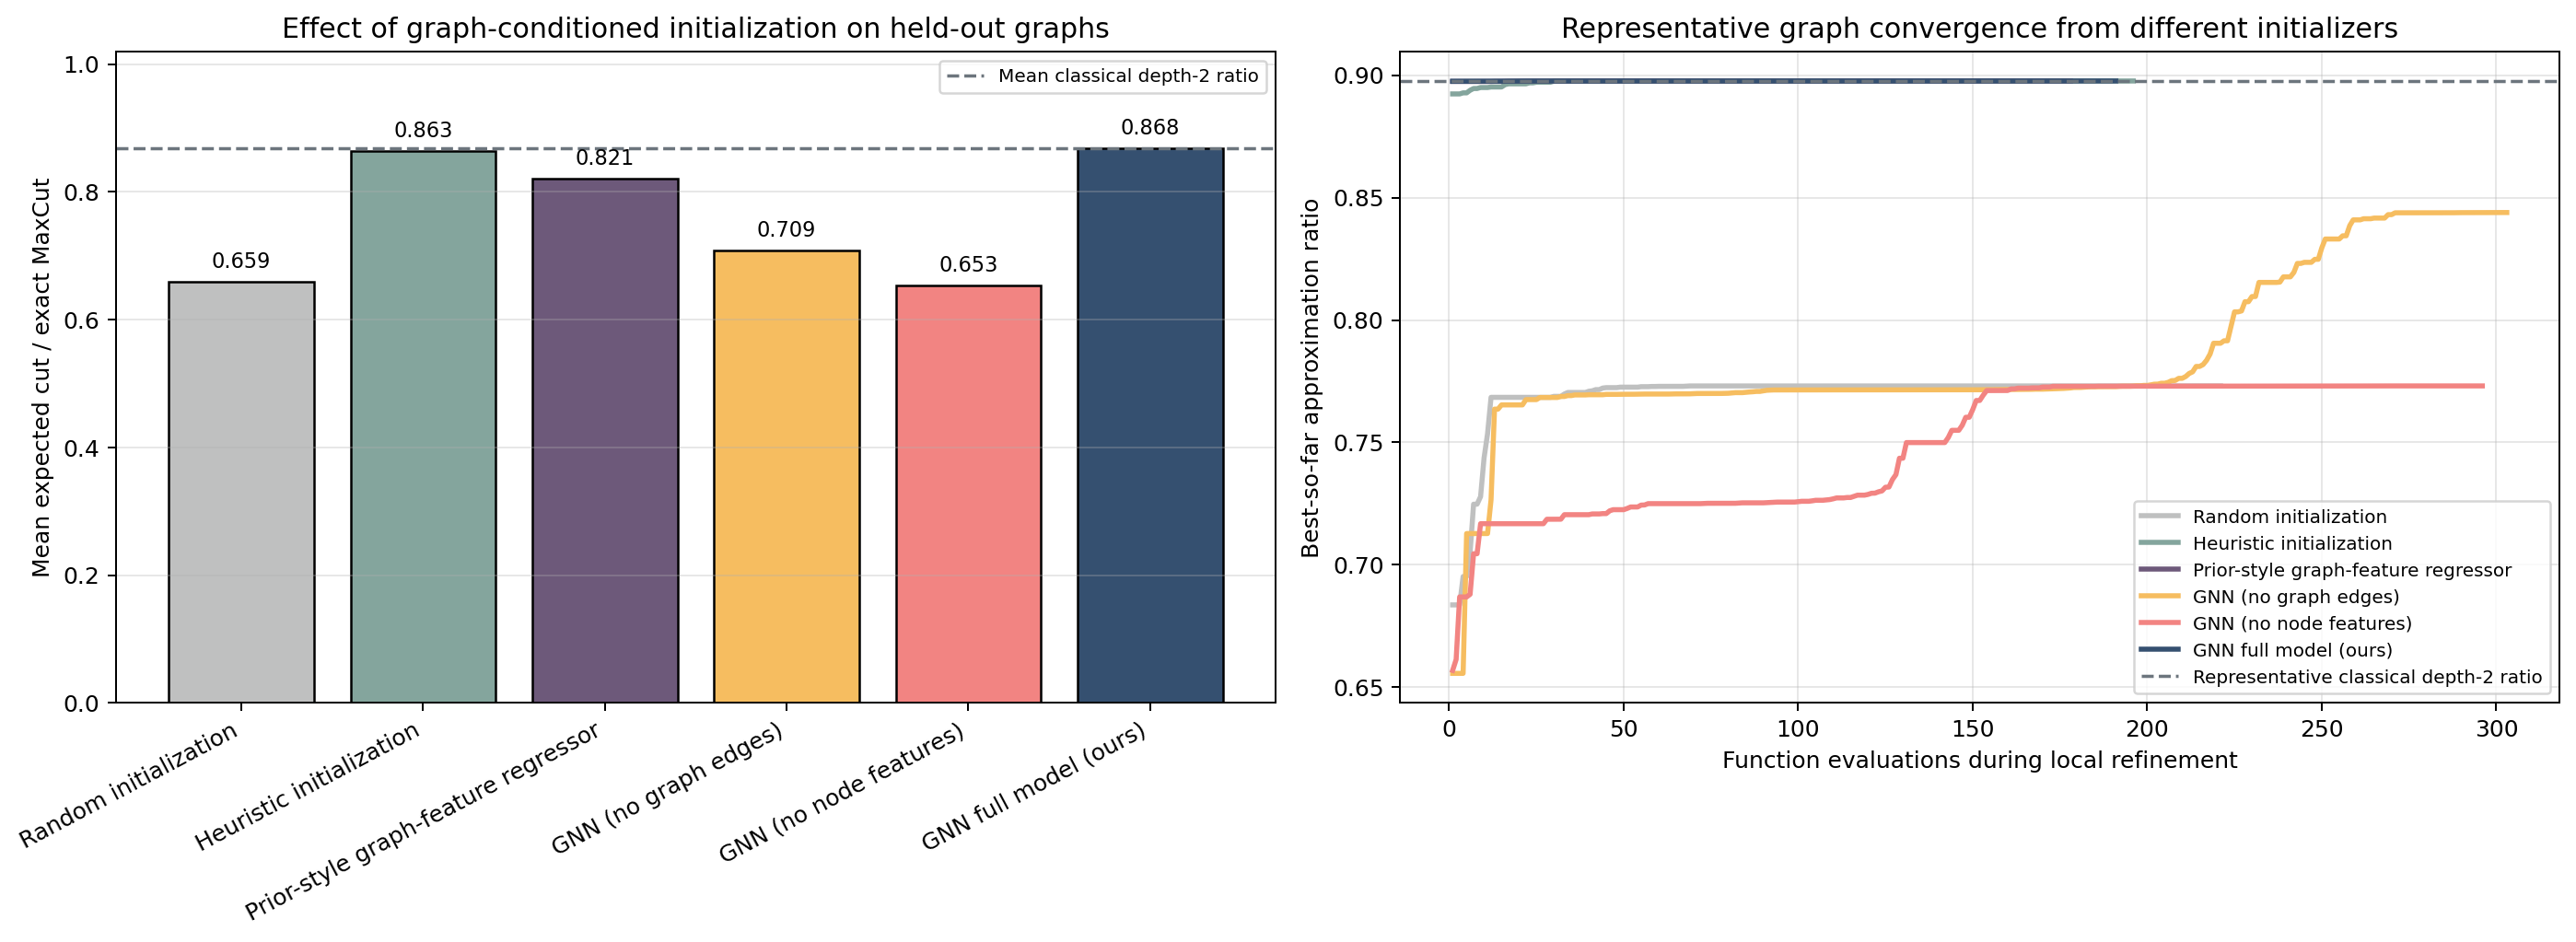
\includegraphics[width=\linewidth]{figures/qaoa_demo_graph_conditioned_initialization.png}
    \caption{Learned initializer comparison and graph ablations. Both topology and node features materially contribute to the final objective value, indicating that the model is not collapsing to a global angle prior.}
    \label{fig:qaoa-ablation}
  \end{minipage}
\end{figure*}

\begin{table*}[t]
\caption{Held-out transcriptomic QAOA benchmark summary.}
\label{tab:qaoa}
\begin{ruledtabular}
\begin{tabular}{lll}
Method & Held-out mean ratio & Interpretation \\
\colrule
Direct classical depth-2 search & 0.8686 & Strongest quality reference, but latency-heavy. \\
Graph-conditioned GNN, depth-2 & 0.8682 & Retains 99.95\% of classical quality with one forward pass. \\
Prior-style learned baseline & 0.8208 & Graph-agnostic learned warm start; weaker than graph conditioning. \\
GNN without graph edges & 0.7086 & Removes message passing; objective quality drops sharply. \\
GNN without node features & 0.6535 & Preserving topology without attributes is insufficient. \\
\end{tabular}
\end{ruledtabular}
\end{table*}

The core optimization result is therefore not that learning beats exact search. It is that a graph-conditioned parameter generator can almost eliminate the online cost of search while preserving nearly all of its quality on held-out, biologically grounded graphs. This is precisely the regime in which graph-conditioned parameterization is useful: a repeated family of related graphs where test-time search is the bottleneck and exact downstream evaluation is still available for auditing.

\section{Instantiation II: Clinical Risk Modeling on CTG Similarity Graphs}
The biomedical branch uses the UCI cardiotocography cohort, a public dataset with 2126 exams and 21 physiologic summary variables extracted from fetal heart rate and uterine contraction recordings. The original three-class label is collapsed into a binary screening task: pathologic versus nonpathologic. The pathologic class is rare, which makes simple accuracy insufficient. The clinically relevant object is a risk surface that can later be thresholded under different operating priorities.

The graph is built with split-first preprocessing. A stratified train-validation-test partition is created before fitting the standardization transform, and a symmetric $k$-nearest-neighbor graph is then constructed on standardized features. This design avoids the common leakage pattern where preprocessing statistics are fit globally before the split. It also exposes a meaningful graph semantics: node neighborhoods correspond to physiologically similar exams, not to arbitrary index structure.

Under the selected operating point reported in the public site and notebook exports, the graph model reaches 98.8\% held-out accuracy, 0.942 balanced accuracy, 0.978 ROC AUC, detects 31 of 35 pathologic cases, and produces one false positive. The strongest calibrated tabular baseline remains slightly better in summary metrics, reaching 99.06\% accuracy and 0.956 balanced accuracy. This narrows the scientific claim. The biomedical branch demonstrates that graph-conditioned parameterization yields a strong, threshold-aware operating point on a patient-similarity graph, but not that graph methods universally dominate tabular learners on this cohort.

\begin{figure*}[t]
  \centering
  \begin{minipage}[t]{0.48\textwidth}
    \centering
    
\includegraphics[width=\linewidth]{figures/bio_demo_heldout_evaluation.png}
    \caption{Held-out evaluation dashboard for the CTG graph model. The paper treats this operating surface, not only the classifier logits, as the primary downstream object.}
    \label{fig:ctg-dashboard}
  \end{minipage}\hfill
  \begin{minipage}[t]{0.48\textwidth}
    \centering
    
\includegraphics[width=\linewidth]{figures/combined_ctg_robustness.png}
    \caption{Fixed-split robustness analysis from the integrated notebook export. Training-seed sensitivity remains modest, supporting the claim that the graph operating point is not a single-seed artifact.}
    \label{fig:ctg-robustness}
  \end{minipage}
\end{figure*}

\begin{table*}[t]
\caption{Held-out CTG benchmark summary at the selected operating point.}
\label{tab:ctg}
\begin{ruledtabular}
\begin{tabular}{lccccc}
Model & Accuracy & Balanced accuracy & ROC AUC & TP / 35 & FP \\
\colrule
Logistic regression & 94.1\% & 0.916 & 0.984 & 31 & 21 \\
XGBoost & 98.8\% & 0.955 & 0.992 & 32 & 2 \\
Calibrated LightGBM & 99.06\% & 0.956 & 0.991 & 32 & 1 \\
ResidualClinicalGCN & 98.8\% & 0.942 & 0.978 & 31 & 1 \\
\end{tabular}
\end{ruledtabular}
\end{table*}

The graph model is therefore best interpreted as a competitive decision-support surface rather than as a universal tabular replacement. Its distinctive value lies in graph-aware evidence aggregation, neighborhood-structured reasoning, and a unified methodology that is also meaningful in the optimization branch. The interface claim survives even when the strongest tabular comparator retains a slight performance edge.

\section{Experimental Protocol and Evaluation Logic}
The two branches share neither labels nor losses, but they do share an evaluation philosophy. In both cases, the parameterization emitted by the graph model is assessed through a downstream system that is independently meaningful. The QAOA branch uses exact MaxCut and exact statevector evaluation on small graphs so that every quality claim is auditable. The biomedical branch uses split-safe preprocessing, held-out operating-point reporting, and comparison against strong tabular baselines so that every claim is operationally interpretable.

\subsection{Transcriptomic branch protocol}
The transcriptomic branch uses a representative full-cohort graph together with 24 adaptation graphs and six held-out graphs. Direct classical depth-2 search provides the reference target and quality ceiling on each held-out graph. The graph model is trained only on the adaptation family. Quality is summarized through mean held-out approximation ratio, retention relative to direct search, and runtime difference between repeated optimization and single-pass inference.

\subsection{Biomedical branch protocol}
The CTG branch uses a 68/12/20 split with standardization fit only on training rows. The $k$-nearest-neighbor graph is constructed after split-safe standardization. Class-weighted training addresses pathologic rarity. Validation data determines the deployed threshold. The held-out test set is used once for the final operating-point report. Metrics include accuracy, balanced accuracy, ROC AUC, precision, recall, and false positives.

\subsection{Why these protocols match the interface claim}
Graph-conditioned parameterization is meaningful only if the downstream consumer is part of the evidence. That means the evaluation cannot stop at angle regression loss or cross-entropy. The optimization branch must show objective retention and latency. The screening branch must show threshold-aware behavior under imbalance. Both branches therefore emphasize decision-surface metrics rather than proxy losses.

\section{Results}
Across the six held-out transcriptomic graphs, the graph-conditioned model reaches 0.8682 mean approximation ratio versus 0.8686 for direct classical search. The absolute gap is 0.0004. Reported on the project website, this corresponds to 99.95\% quality retention while reducing median inference time from 675.9 ms to 0.256 ms. The strongest interpretation is not that learning beats search. It is that graph-conditioned inference renders per-instance search almost unnecessary in this small exact-simulation regime.

The learned baseline comparison is equally important. The prior-style graph-agnostic regressor reaches 0.8208 mean held-out ratio. The graph-conditioned model improves that to 0.8682. The relative lift is therefore substantial, and the ablation study shows that both message passing and node features contribute materially. Removing graph edges drops the mean ratio to 0.7086; removing node features drops it to 0.6535.

The biomedical branch reaches a strong graph operating point: 98.8\% held-out accuracy, 0.942 balanced accuracy, and one false positive. This places the graph model above weaker clinical baselines and near the strongest tabular ones. Calibrated LightGBM remains slightly better on this split, which is an honest and important result. It narrows the claim from superiority to competitiveness, while preserving the broader argument that graph-conditioned parameterization remains useful when the downstream object is a thresholded risk surface.

The most important result of the paper is not any single scalar metric. It is the alignment between branches at the level of interface. In the optimization branch, the graph model emits control variables for a downstream quantum-style objective. In the biomedical branch, the graph model emits risk variables for a downstream policy. In both cases, the scientific object is the graph-generated parameterization and its consequences.

\section{Discussion}
The paper makes a methodological claim supported by two case studies. This is both a strength and a limit. It is a strength because it avoids overclaiming transfer or joint training that the repository does not support. It is a limit because the work is not a massive benchmark sweep. The optimization branch remains in a small exact-simulation regime. The clinical branch is retrospective and public-cohort specific. Neither branch supports deployment claims on its own.

Those limitations are not incidental. They are part of why the results are interpretable. Small transcriptomic graphs make exact MaxCut and exact statevector evaluation feasible, which makes the QAOA evidence unusually auditable. A fixed public CTG cohort makes graph-versus-tabular benchmarking and threshold analysis reproducible. The cost of that rigor is that the paper cannot claim external cohort transport, hardware-scale quantum advantage, or a universal win for GNNs over all clinical tabular baselines.

\section{Limitations, Ethics, and Reproducibility}
The QAOA branch studies depth-2 circuits on small graphs under exact statevector simulation. This is the correct regime for auditability but not for claims about large-scale hardware deployment. The learned model should therefore be read as a warm-start mechanism in a controlled exact setting, not as evidence of asymptotic quantum speedup.

The CTG branch is a retrospective study on a public cohort. It does not address prospective integration into clinical workflow, site shift, fairness assessment, or liability-sensitive deployment. The strongest tabular baseline also remains slightly better on the reported split. The graph result is best interpreted as evidence that graph-structured patient similarity can support a strong operating point under strict evaluation, not as a final clinical product.

The biomedical analysis is framed as decision support rather than autonomous diagnosis. Thresholds are selected on validation data only. The reported false-positive and false-negative tradeoffs are exposed rather than hidden behind a single summary statistic. This is important because screening systems produce interventions, not only predictions.

\section{Conclusion}
This paper introduced graph-conditioned parameterization as a compact formulation for graph models whose outputs parameterize downstream computation rather than terminating in standalone predictions. We instantiated the idea in two settings: transcriptomic depth-2 QAOA angle prediction and cardiotocography graph risk scoring. The optimization branch showed near-parity with direct classical search at a fraction of the inference cost. The biomedical branch showed a strong graph operating point under stricter tabular benchmarking, while also clarifying that the strongest calibrated tabular model remains slightly better on this cohort.

The broader claim is therefore pragmatic rather than rhetorical. Graph models should sometimes be evaluated by the decision variables they generate and by what those variables enable downstream. When that is the actual engineering role of the model, graph-conditioned parameterization provides a sharper language for method design, benchmarking, and interpretation.

\nocite{zhao2020,alon2021,topping2022,thekumparampil2018,klicpera2019diffusion,brody2022,knyazev2019,li2019deepgcn,cai2020,dwivedi2021bresson,he2017workshop}

\bibliographystyle{apsrev4-2}
\bibliography{refs}

\end{document}